\subsection{Channel models}

The Schr\"odinger equation and the Manakov equation are two commonly used mathematical models for describing the behavior of light propagation in a single-mode optical fiber, including the effects of dispersion and nonlinearity.

The Schr\"odinger equation is a well-known equation that describes the behavior of wave-like phenomena in quantum mechanics. In the context of optical fiber transmission, the Schr\"odinger equation is used to describe the evolution of the slowly varying optical field envelope, $A(z,t)$, in the presence of dispersion and nonlinearity. The general form of the Schr\"odinger equation for a single-polarization signal is as follow:

\begin{equation}
	\frac{\partial A }{\partial z} = - \frac{\alpha}{2} A - i \frac{\beta_2}{2} \frac{\partial^2 A}{\partial t^2} + i \gamma |A|^2 A {,}
\label{eq:nlse}
\end{equation}

where $z$ represents the distance along the fiber, $t$ is time, $\beta_2$ is the group velocity dispersion (GVD) parameter, $\gamma$ is the nonlinear coefficient, and $A$ is the complex envelope of the optical field.

The Manakov equation is a more complex model that is used to describe the behaviour of light propagation in a two-polarisation optical fiber. It considers the effects of polarization-mode dispersion and nonlinear interactions between the two polarizations. The Manakov equation for a two-polarization signal is as follows:

\begin{gather} 
\frac{\partial A_x}{\partial z} = -\frac{\alpha}{2} A_x - i\frac{\beta_2}{2}\frac{\partial^2 A_x}{\partial t^2} + i\gamma\frac{8}{9}\left(|A_x|^2 + |A_y|^2\right) A_x {,} \nonumber \\
\frac{\partial A_y}{\partial z} = -\frac{\alpha}{2} A_y - i\frac{\beta_2}{2}\frac{\partial^2 A_y}{\partial t^2} + i\gamma\frac{8}{9}\left(|A_x|^2 + |A_y|^2\right) A_y {,}
\label{eq:manakov}
\end{gather}
where $A_x$ and $A_y$ are the complex envelopes of the two polarizations.





\subsection{Basics of the Inverse Scattering Transform }
We briefly remind in this section basics of the inverse scattering method~\cite{ZakharovShabat1972}.
% Channel description

% Signal propagation is modelled by the nonlinear Schr\"odinger equation (in the scalar case, when the signal is transmitted through single polarization):

% \begin{equation}
% 	i \frac{\partial Q}{\partial Z} - \frac{\beta_2}{2} \frac{\partial^2 Q}{\partial T^2} + \gamma |Q|^2 Q = 0 {.}
%     \label{eq:GNLSE}
% \end{equation}
% Here $Q$ is a complex envelope field that describes the optical signal, $Z$ is a distance (e.g. in $km$), $T$ is time (e.g. in $ps$), $\beta_2$ (in $ps^2/km$) is the group velocity dispersion parameter and $\gamma$ (in $W^{-1} km^{-1}$) is the nonlinear Kerr coefficient.


\begin{figure}[!bp]
	\centering
	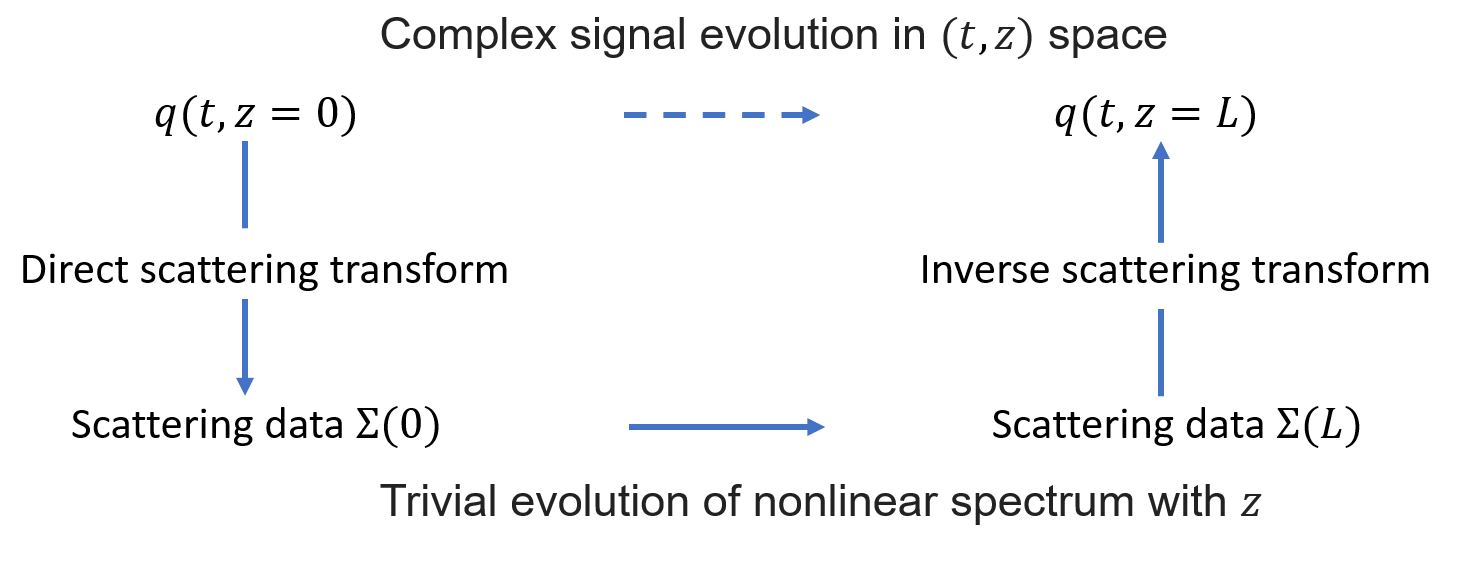
\includegraphics[width=0.7\linewidth]{images/window/IST_scheme.png}
	\caption{Schematic depiction of nonlinear Fourier Transform (NFT) processing}
	\label{fig:IST}
\end{figure}

The nonlinear Schr\"odinger equation (NLSE) (\ref{eq:nlse}) belongs to the class of the so-called integrable nonlinear partial differential equations that can be integrated by the inverse scattering transform (IST) method, also known as the nonlinear Fourier transform (NFT)~\cite{ZakharovShabat1972, Ablowitz1981}.
The inverse scattering transform allows one to find the evolution (with $z$) of the signal $q(t,z)$ described by the NLSE channel by solving two linear problems instead of solving the nonlinear partial differential equation. A complex signal evolution governed by NLSE is replaced by 3 steps (see Fig.~\ref{fig:IST}):
\begin{enumerate}
    \item direct (linear) transform from $q(t,z=0)$ to the so-called scattering data $\Sigma(0)$ (nonlinear spectrum of the initial signal)
    \item trivial evolution of the nonlinear spectrum with z, and
    \item inverse (linear) transform to restore signal $q(t,z)$ at any desired propagation distance $z$.
\end{enumerate}
% We do describe here all mathematical details as they are comprehensively presented in \cite{Optica}. 
The IST/NFT method is similar to standard Fourier approach for the solution of linear evolution equations: present initial field in the spectral domain, consider trivial evolution of each spectral harmonic, reconstruct evolved signal from the spectral components known for any propagation distance.


Direct NFT corresponds to solving the Zakharov-Shabat spectral problem (ZSSP). We consider here ZSSP problem for the initial signal $q(t,z=0)$: 
\begin{equation}
\left\{
\begin{aligned}
	- \partial_{t} \psi_1 + q(t,0) \psi_2 = i \xi \psi_1 \\
	\partial_{t} \psi_2 + q^{*}(t,0) \psi_1 = i \xi \psi_2 \\
\end{aligned}
\right.
\label{eq:ZS}
\end{equation}
where $q(t,z=0)=q_{0}(t)$ is the "potential" --- initial distribution of the signal to be transmitted, $\psi_{1,2}$ is a vector eigenfunction and $\xi = \lambda + i \zeta$ --- spectral parameter defined on a complex plane.

To determine the nonlinear Fourier spectrum associated with the signal $q(t,z)$, we need to find the special solution $\Phi(t,\xi)$ of Eq. (\ref{eq:ZS}), called Jost function, imposing the special asymptotic condition at the trailing end of the pulse:
\begin{equation}
\Phi(t,\xi)\equiv\left(\begin{matrix}\phi_1\\ \phi_2\end{matrix}\right)
\xrightarrow[t\rightarrow-\infty]{} \left(\begin{matrix}e^{-i\xi t}\\ 0\end{matrix}\right).
\label{eq:asy}
\end{equation}
The nonlinear Fourier pulse decomposition consists in finding the continuous and discrete components of the nonlinear Fourier spectrum associated with the localised signal $q(t,z)$. This means that we will need to use burst-mode transmission --- intervals with the information signal $T_{burst}$ and guard intervals with no signals in between $T_{guard}$. One of the goals in this project is to find out how large the ratio of $T_{burst}/T_{guard}$ can be, at which algorithms of IST/NFT will still work. The core part of IST/NFT is the computation of the scattering coefficients, $a(\xi) \in \mathbb{C}$ and $b(\xi) \in \mathbb{C}$, defined through the Jost solution $\Phi(t,\xi)$ as follows
\begin{equation}
a(\xi)=\lim_{t\rightarrow+\infty}\phi_1(t,\xi) e^{i\xi t},
\qquad b(\xi)=\lim_{t \rightarrow+\infty}\phi_2(t,\xi) e^{-i\xi t},
\label{eq:ab}
\end{equation}
where $\xi \in \mathbb{R}$. The scattering coefficients for the considered (anomalous dispersion) NLSE satisfy:
\begin{equation}
|a(\xi)|^2 + |b(\xi)|^2 \equiv 1.
\label{eq:quad_inv}
\end{equation}
The continuous part of NF spectrum is generally defined by the ratio of quantities $b$ and $a$ from (\ref{eq:ab}):
\begin{equation}
\label{r}
r(\xi)=b(\xi)/a(\xi), \qquad r(\xi) \in \mathbb{C},
\end{equation}
where $r(\xi)$ is often refereed to as the reflection coefficient.
For the parameter $ \xi = \zeta $, for $ \mathrm{Im} \ \zeta> 0 $, the zeros of the coefficient $ a(\zeta_n) $ determine the discrete spectrum $ \zeta_n $, for $ n = 1... N $, $ N $ is the number of discrete eigenvalues and the parameter.
\begin{equation}
    c_n(z) = c(\zeta_n, z) = \frac{b(\zeta_n)}{a'(\zeta_n)} {,} \quad \text{where} \quad 
    a'(\zeta_n) = \frac{\partial a(\zeta)}{\partial \zeta}|_{\zeta = \zeta_n} {,}
    \label{eq:scat_sol}
\end{equation}
is a phase coefficient, which defines complex phase shift for each soliton.
The coefficients obtained are the so-called "scattering data", which determine the initial potential $q_0 (t)$.

The dependence of the scattering data on $z$ can be represented in the form:
\begin{equation}
    r(\xi,z) = r(\xi,z_0) e^{-2i \xi^2 (z - z_0)} {,} \quad 
    c_n(z) = c_n(z_0) e^{-2i \zeta_n^2 (z - z_0)} {.}
\end{equation}

The scattering data forms the core $ \Sigma (z) = \Sigma_{dis} (z) + \Sigma_{con} (z) $, sum of the discrete and continuous nonlinear spectra, where
\begin{equation}
    \Sigma_{dis}(z) = \sum_{n}^{N} c_n(z) e^{-i \zeta_n z} {,}
    \label{eq:kernel_sol}
\end{equation}
\begin{equation}
    \Sigma_{con}(z) = \frac{1}{2\pi} \int_{-\infty}^{+\infty} d\xi r(\xi, z) e^{-i \xi z} {.}
    \label{eq:kernel_rad}
\end{equation}
Here $N$ is a total number of discrete eigenvalues in signal.

The final step of the NFT is to restore the signal from the scatter data. In order to restore the signal $q (t, z)$ at the required point $z$, the obtained core $\Sigma (z)$ must be substituted into a pair of integral equations that are called "Gelfand-Levitan-Marchenko equations"\ (GLM):
\begin{equation}
    A_1^{*}(t,s)+\int_{-s}^{t} \Sigma(s+\tau) A_2(t,\tau) d\tau = 0 {,}
    \label{eq:glm_1}
\end{equation}
\begin{equation}
    -A_2^{*}(t,s)+\int_{-s}^{t} \Sigma(s+\tau) A_1(t,\tau) d\tau + \Sigma(t+s) = 0 {,}
    \label{eq:glm_2}
\end{equation}
where the parameters are within $ -t \le s <t $ and $ 0 \le t \le T $, $ \Sigma (t) \equiv \Sigma (z = 0, t) $. A pair of functions $A_1$ and $A_2$ constitute a solution to the GLM equations. After finding the functions $A_1$ and $ A_2 $, the signal is restored by
simple formula
\begin{equation}
    q(z,t)= -2 A_2^{*}(t,t) {.}
    \label{eq:glm_q}
\end{equation}



\subsection{Sliding window processing}
\subsubsection{Conventional window}

\begin{figure}[!bp]
\center{
    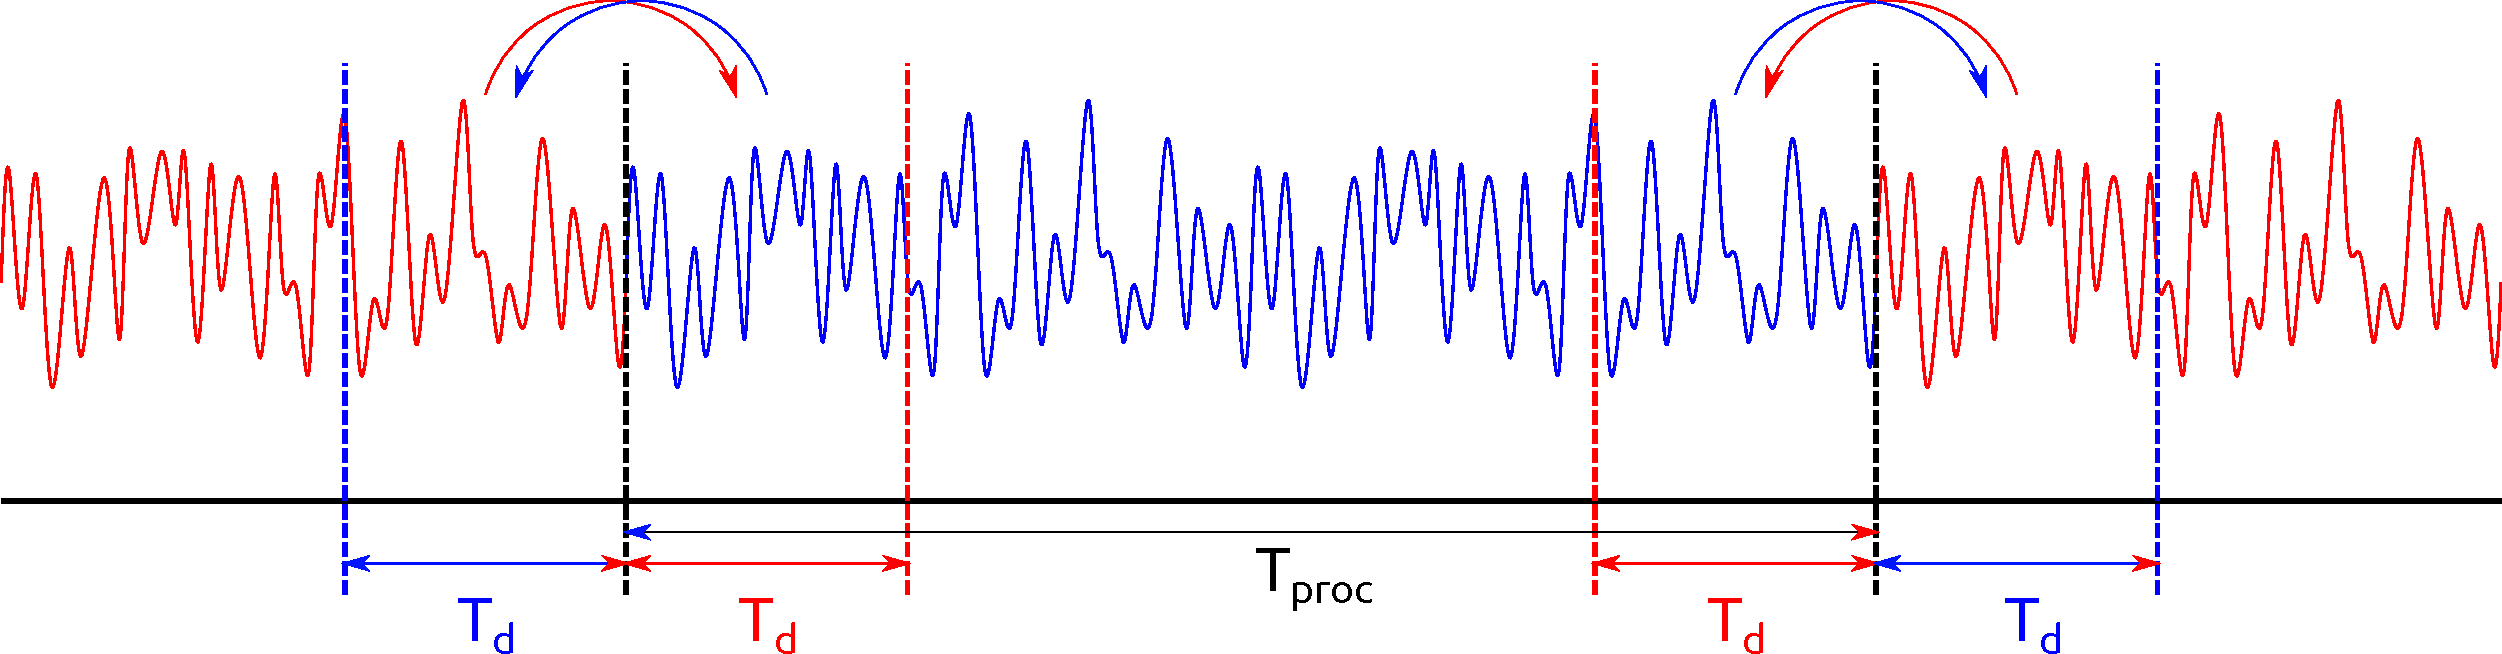
\includegraphics[width=1\linewidth]{images/window/periodical_signal_short.pdf}
}
\caption{Signal decomposition}
\label{fig:periodical_signal}
\end{figure}

Let's consider a continuous signal, denoted as $A(z = L, t)$, which we intend to process using the NFT with vanishing boundary conditions. To clarify, the notation for $A$ in equation~(\ref{eq:nlse}) remains consistent throughout. However, in the case of the Manakov equation, $A$ represents the vector $[A_x, A_y]$, and all operations are independently applied to each component.

To achieve accurate processing, it is crucial to account for dispersion that occurs during signal propagation. Dispersion leads to neighboring symbols overlapping and distorting, potentially compromising the accuracy of subsequent signal processing steps.

To address this challenge, we introduce side dispersion intervals, denoted as $T_d$, on both the left and right sides of a designated processing interval, referred to as $T_{proc}$ (see Fig.~\ref{fig:periodical_signal}). This approach ensures that the processing interval effectively captures the nonlinear distortions in the signal while allowing the signal to be influenced only by the effects of the side dispersion intervals, rather than other parts of the signal beyond the designated interval.

The length of the dispersion interval, $T_d$, depends on the propagation distance and can be approximated by:

\begin{equation}
    T_d = \beta_2 \times \Omega \times L {,}
\end{equation}
where $\beta_2$ is the group velocity dispersion parameter of the fiber, $L$ is the propagation distance, $\Omega$ is the signal bandwidth.

To cut the signal we define the window function $W(t)$ as a combination of Heaviside step functions that selects the time interval for processing:
\begin{equation}
W(t, t_w) = \begin{cases}
1, & t_w - T_d \leq t \leq t_w + T_{proc} + T_d, \\
0, & \text{otherwise} {,}
\end{cases}
\end{equation}
where $t_w$ corresponds to the time parameter associated with the current position of the processing window.

Then, we take a signal $A_w(t)$ inside this $T_d + T_{proc} + T_d$ window defined by 
\begin{equation}
    A_w(t, t_w) = A(t) W(t, t_w)
\label{eq:window}
\end{equation}
and use NFT. 
It will restore the initial transmitted signal $A_w(z = 0, t, t_w)$, but side intervals $T_d$ will be corrupted due to the fact that we windowed the signal and lost information about the previous and following intervals. So we cut again and take only the $T_{proc}$ interval:
\begin{equation}
W_{proc}(t, t_w) = \begin{cases}
1, & t_w \leq t \leq t_w + T_{proc}, \\
0, & \text{otherwise} {.}
\end{cases}
\end{equation}
It will have all the necessary information about nonlinear distortions and other effects from the side intervals $T_d$. It exclusively considers these effects and disregards any influence from previous or subsequent intervals.

The resulting solution can be expressed by the following equation:

\begin{equation}
A_w(z = 0, t, t_w) = W_{proc}(t, t_w) \cdot \mathrm{NFT}[A_w(z = L, t, t_w)] {.}
\end{equation}

In this equation, $A_w$ represents the value at the output of the processing window. It's calculated as the product of the processing window function, $W_{proc}(t, t_w)$, and the nonlinear Fourier transform of the input signal, which is the product of $A(z=L,t)$ and the window function $W(t, t_w)$ at the fiber's end, located at $z=L$. We can iterate this procedure by incrementing $t_w$ with the value of the processing interval $T_{proc}$. This allows us to repeat the process for the next position of the processing window.

While this method can be effective in certain scenarios, its numerical accuracy may not always be optimal. To enhance the precision of the calculation methods, it might be necessary to insert zero intervals on both sides of the processing signal. Furthermore, dealing with a signal of high average power can result in a significant number of soliton components, making the computational analysis challenging. Particularly, the computation of nonlinear spectrum phases for solitons can be highly unstable, and as the power of the solitons increases, the numerical calculations may become less reliable.

To address these challenges and enhance the stability of numerical calculations, we propose a more advanced method, which will be elucidated in the subsequent section.

\subsubsection{Compensated window}

As previously discussed, the dispersion occurring during signal propagation leads to the overlapping and distortion of neighboring symbols. This can significantly compromise the accuracy of subsequent signal processing. However, we can mitigate this issue by leveraging our understanding of the propagation model, such as the Schr\"odinger equation for single polarization or the Manakov equation for dual polarization. We achieve this by effectively "compressing" the signal before processing through the compensation of chromatic dispersion. While this operation restores symbols to their initial positions, it does introduce some level of corruption due to nonlinear effects during propagation. Following dispersion compensation, we proceed to window the signal and subsequently decompensate the dispersion to obtain a processed signal ready for analysis using the NFT.

To initiate the process, we compensate for the dispersion across the entire signal using the equation:

\begin{equation}
A_{CD}(t) = F^{-1}F[A(t)]e^{i\phi_{CD}(\omega)} {,}
\end{equation}

Here, $F[\cdot]$ and $F^{-1}[\cdot]$ represent the forward and inverse linear Fourier transforms, respectively. The phase shift $\phi_{CD}$ can be readily determined from equations~(\ref{eq:nlse}) and~(\ref{eq:manakov}) by setting $\gamma = 0$ and $\alpha = 0$. It is given by:

\begin{equation}
\phi_{CD} = -\frac{\beta_2}{2} \omega^2 L {.}
\label{eq:cdc_phase}
\end{equation}
%
Here, $\beta_2$ denotes the second-order dispersion coefficient of the fiber, $\omega$ is the angular frequency, and $L$ represents the length of the fiber.

Subsequent to dispersion compensation, we apply the same window operation as described in equation~(\ref{eq:window}). We then proceed to decompensate the dispersion using the same phase shift~(\ref{eq:cdc_phase}). This results in:

\begin{equation}
A_{w, CD}(t, t_w) = A_{CD}(t) W(t, t_w) {,}
\end{equation}

\begin{equation}
A_{\tilde{w}}(t) = F^{-1}F[A_{w, CD}]e^{-i\phi_{CD}(\omega)} {,}
\end{equation}

The final solution for a processing window using the dispersion-compensated window mode is depicted below:

\begin{equation}
A_{\tilde{w}}(z = 0, t, t_w) = W_{proc}(t, t_w) \cdot \mathrm{NFT}[A_{\tilde{w}}(z = L, t, t_w)] {.}
\end{equation}

Similar to the conventional window mode, we can increment $t_w = t_w + T_{proc}$ to continuously process the full signal.

For the practical implementation of the signal recovery process using the NFT, we need to introduce additional variables. To construct a time window for the recovery of the full signal, we employ the following expression:

\begin{equation}
T_w = T_{proc} + 2 \cdot (R_d \cdot T_d + T_z) {;} \quad T_{proc} = N \cdot T_s {.}
\end{equation}
%
Here, $T_{proc}$ represents the processing interval with $N$ symbols, and $T_s$ denotes the duration of one symbol interval. The term $R_d$ acts as a scale factor for the dispersive length, while the term $T_z$ corresponds to the number of additional empty symbol slots added to each side of the processing interval, enhancing the accuracy of the NFT.

The final procedure for processing a continuous WDM signal with NFT can be summarized as follows:

\begin{enumerate}
\item Compensate for the dispersion of the propagated signal without additional equalization.
\item Define and isolate the required window within the compensated signal.
\item Decompensate the dispersion for the windowed signal.
\item Process the signal within the window using NFT (given that it is already localized).
\item Collect the full signal for further analysis.
\end{enumerate}


